
\documentclass[onehalf,11pt]{beavtex}
\title{Energy-Aware Gossip Techniques for Wireless Broadcasting}
\author{Tingzhi Li}
\degree{Master of Science}
\doctype{Thesis}
\department{Electrical Engineering and Computer Science}
\depttype{School}
\depthead{Head}
\major{Electrical and Computer Engineering}
\advisor{Bechir Hamdaoui}
\submitdate{December 8, 2016}
\commencementyear{2017}
\abstract{The current state of research on gossip techniques for wireless broadcasting is very limited because past research efforts have mostly focused on using gossip techniques for multicast communication. On the other hand, those research efforts that have focused on using gossip techniques for wireless broadcast communications ignore energy efficiency and network lifetime. With the emergence of Internet of Things (IoT) devices, known with their limited energy and processing resource capabilities, energy consumption is becoming more and more important to account for when designing wireless broadcasting protocols. In this thesis, we propose a new energy-aware broadcasting protocol for wireless adhoc networks. Specifically, the proposed protocol dynamically adapts the fanout parameter based on wireless nodes' remaining energy to prolong the lifetime of the network. Our simulation results show that our proposed energy-aware gossip protocol outperforms existing approaches by achieving fast message broadcasting times while extending the nodes' battery lifetime.}
\acknowledgements{
I would first like to thank my advisor Dr. Bechir Hamdaoui of the School of Electrical Engineering and Computer Science at Oregon State University. The door to Professor Hamdaoui office was always open whenever I had a question about my research or writing. I would like to express my gratitude to him for the useful remarks and engagement through the researching and writing process of this master thesis. 
	
I would also like to thank Sherif Abelwahab for introducing me to the topic, providing great suggestions and answering my questions in many discussions. This research started as a team project in Advanced Computer Network class. Here, I would also like to acknowledge Marco Falke and Jinming Mu as initial project team members who participated in this project and in many ways shaped my research today.
	
Finally, I must express my very profound gratitude to my amazing parents Min Li, and Suling Han for their unfailing support and encouragement throughout my years of study abroad and through the process of researching and writing this thesis. This accomplishment would not have been possible without them. Moreover, I would like to thank my girlfriend Kendall Bailey for her unwavering support both during graduate school and my life.
}

%\usepackage{algorithm}
%\usepackage{algorithmic}

\usepackage{graphicx}
\usepackage{listings}
\usepackage{verbatim}
\usepackage{color}
\usepackage{fancyvrb}

\newcommand{\gp}{gossip protocol}
\newcommand{\pog}{Probability of Gossip}
\newcommand{\msgs}{messages}
\newcommand{\msg}{message}
\newcommand{\pp}{push-pull}
\newcommand{\gn}{gossip node}
\newcommand{\gns}{gossip nodes}
\newcommand{\im}{implementation}
\newcommand{\wf}{WiFi}
\newcommand{\sn}{source node}
\newcommand{\br}{broadcast}
\newcommand{\nl}{Network Lifetime}
\newcommand{\ambt}{Average Message Broadcast Time}
\newcommand{\anl}{Average Network Lifetime}
\newcommand{\aec}{Average Energy Consumption}
\newcommand{\ao}{Average Overhead}

\begin{document}
\maketitle

\mainmatter

\chapter{Introduction} \label{Chapter1}
%\lhead{Chapter 1. \emph{Introduction}} % Write in your own chapter title to set the page header

Along with the development of the information technology, the price of the broadband connectivity becomes affordable. Devices are trending to be smaller and more powerful. People start to explore ways to connect devices to the network for better control and monitor the status of them. Devices such as smart phone, smart watch, smart thermostats, and radio-frequency identification (RFID) tags are able to connect to a network and these devices can communicate with each other. If these devices are connected to the Internet as well, we call them the \textit{Internet of Things}. There is no doubt that IoT is an innovative paradigm \cite{Atzori} because this idea combined the Internet with our everyday gadgets. Either from the perspective of private user or from the perspective of business user, there are infinite possible ways to exploit IoT. As of today, research in the area of IoT is emerging rapidly and many open questions remain to be answered.

Many application services that IoT devices can provide rely on a network broadcast protocol to disseminating information \cite{smart}. For example, IoT devices firmware update package can be broadcast among devices in a distributed manner. However, the main challenge here is that IoT devices are often resource limited meaning they have limited bandwidth and energy, and restricted by their mobility. Due to the characteristics of IoT devices, topology of physical network formed from IoT devices is often dynamic. Therefore, a scalable, robust, and fault-tolerant broadcast protocol is needed for these dynamic networks. Flooding is consider to be the simplest broadcast protocol but it is not suitable. This is because flooding result in excessive overhead, media contention, and packet collision \cite{tseng2002broadcast} which would severely deplete devices' precious battery power. Gossip techniques instead offer a relatively simple, robust, fast and probabilistic approach. This technique is inspired by the form of gossip seen in social network.

Besides gossip techniques, several deterministic approaches have been proposed which aim to reduce overhead by shifting \msg ~forward responsibility to a subset of nodes in the network \cite{smart}. However, there are two main problems for these approaches. First, if any node in the subset fails, nodes that depend on it will not be able to receive new \msgs \cite{smart}. Second, the energy nodes in those subset will be depleted sooner than other nodes that are not the subset \cite{smart}.

To properly define a variation of gossip technique, three main parameters need to specified. They are \emph{\pog}, \emph{Fanout}, and \emph{Message Live Time}. With gossiping, nodes in the network have to forward the \msg ~with probability $p_{gossip} \leq 1$ \cite{smart}. The idea is that a message can be broadcast successfully without every nodes' participation \cite{smart}. This approach can achieve a lower overhead because only a portion of the nodes participated in gossiping. However, the right $p_{gossip}$ can be difficult to choose because global topology information is needed. Furthermore, an optimal $p_{gossip}$ can become sub-optimal over time \cite{smart}. 

In terms of energy consumption, several adaptive energy based probabilistic schemes have been proposed. Most of them focused on dynamically adjusting $p_{gossip}$ based on energy level related parameters. D. Nitnaware et. al proposed an adaptive \gp ~based on node's energy level. When a node's energy level is above threshold, it will gossip the \msg ~with a fixed $p_{gossip}$. When a node's energy is below the threshold, it will drop the \msg. For a special case where a node only has one neighbor, the \emph{\pog} is set to be 1 regardless of its energy level \cite{2015survey}. This approach adjusts \emph{\pog} in a very coarse manner since a node would only operate in one of two states: gossip with a fixed probability, or drop incoming new \msgs. In \cite{nitnaware2010energy}, node's remaining energy fraction is used directly as \emph{\pog}. Clearly, this is more fine-tuned than \cite{nitnaware2009performance}.

However, none of these efforts focused on another key gossip technique parameter: \emph{Fanout}. From our observation, for any given \emph{\pog}, higher \emph{Fanout} setting allows nodes to contact more neighbors each round thus achieve a faster message broadcast time. But higher \emph{Fanout} setting usually is associated with higher energy consumption. On the other hand, lower \emph{Fanout} setting conserves nodes' battery power but takes longer to broadcast a \msg. Our aim in this thesis is to retain the benefit of high \emph{Fanout} setting (fast message broadcast time), and increase the lifetime of the network. Therefore, we proposed a gossip broadcast protocol that can dynamically adjust \emph{Fanout} parameter based on each gossip node's remaining energy level.

The rest of this thesis is organized as follows. We present related work in Chapter 2. Chapter 3 describes the classic \gp, our basic \pp ~\gp, and our proposed energy-aware adaptive fanout extension. Chapter 4 presents the implementation of our energy-aware \gp. We present performance evaluation in Chapter 5, and conclusion and future work in Chapter 6.

%The gossip protocol could be used to build routing table[?], perform multicast[?], or in this case, perform broadcast.

% gossip techniques can be used to design routing protocol, multicast, broadcast.

%Some proposed a event counter based scheme to combat this issue. The gist of that shceme is that if a node overheard the same messages $a$ times and $a > b$ were $b$ is the threshold, it would not gossip its latest message this time. Some even went a step further, they tried to identify the dependency among a node and its neighbors and dynamically adjust gossip probability based on collected information.

%As we are moving to an IoT and mobile devices dominated world, energy conservation become more and more important as to overall user experience or network survival time. 

\chapter{Related Work} \label{Chapter2}
%\lhead{Chapter 2. \emph{Related Work}} % Write in your own chapter title to set the page header

Over the years, gossip techniques have proven to be the corner stone for building scalable and robust distributed computer network systems. This technique is often used to design multicast protocol \cite{gupta2002efficient} \cite{gossip} , routing protocol, and broadcast protocol. Demers et. al \cite{demers1987epidemic} demonstrated the advantages of deploying this technique in corporation for database maintenance in the early days. In recent years, this technique has been utilized in wired networks \cite{birman1999bimodal} as well as in wireless networks. Many proposed schemes whether is for wired networks or is for wireless networks, all focused on optimizing protocol overhead, or energy consumption. The metrics they used include network density, or nodes' energy level. 

In wired network domain, it has being used for peer-to-peer network \cite{gupta2002efficient}. In wireless network domain, it has being used for mobile ad-hoc networks \cite{chandra2001anonymous} \cite{vahdat2000epidemic}, and wireless sensor networks \cite{levis2004trickle} \cite{miller2005exploring}. There are many proposed schemes that are designed for wired network that uses network information for adaptive gossiping such as \cite{kempe2004spatial} \cite{rodrigues2003adaptive}, but those approaches are not suitable for wireless networks \cite{smart}. 

Some of the basic gossip techniques that are specifically designed for wireless networks includes fixed forward probability scheme \cite{haas2006gossip} where each node has the probability of $p$ to gossip the \msg ~to its neighbor while it has the probability of $1-p$ to not gossip the \msg ~to its neighbor. Because in this paper the authors are designing a routing protocol in a wireless ad-hoc network, each time when a node receives a new \msg, it will only pick one of its neighbors. In other words, the \emph{Fanout} here is set to be 1. The advantage of this proposed scheme is that it is easy to implement in practice. However, due to the dynamic nature of mobile ad-hoc network or wireless sensor network, a fixed forward probability can be difficult to choose. Moreover, even an optimal forward probability may become sub-optimal over time. 

To address the disadvantage of a fixed forward probability scheme, Cartigny et. al \cite{cartigny2003border} proposed a new broadcast scheme for ad-hoc networks that would adjust \emph{\pog} based on number of neighbors a node has. The equation for calculating \emph{\pog} is $p_{gossip}=\frac{k}{n_b}$ where $k$ is the propagation factor and $n_b$ is a node's degree (number of neighbors). The minimum and maximum \emph{\pog} can be adjusted by changing propagation factor. The idea is that a node with more neighbors will have a lower probability to gossip new \msgs ~and vice versa. This scheme reduced overhead by tailoring \emph{\pog} for each node but a suitable $k$ value for various ad-hoc network topologies can still be difficult to choose. 

Another interesting proposed gossip broadcast scheme is called "Smart Gossip" \cite{smart}. It uses "family classification" method to category a node's neighbors. A node's neighbor can be classified in one of three categories: parent, sibling, or child. Intuitively, the more siblings a node has, the lower the \emph{\pog} will be because other siblings may have transmit the new \msg ~to the child \cite{2015survey}. Moreover, \emph{\pog} is proportional to number of children a node has \cite{2015survey}. When a node has no child, the $p_{gossip}=0$. When a node has no siblings but only child, the $p_{gossip}=1$. This advantage of this approach is that it takes nodes dependency into account while gossiping. However, this scheme can be complicated to implement and there is no update after the initial hierarchy establishment \cite{2015survey}.

In terms of reducing energy consumption while using gossip techniques, Nitnaware et. al \cite{nitnaware2009performance} proposed a simply scheme by defining a \emph{Energy Level Threshold}. When a node's energy level drops below the threshold, this node will not gossip new \msgs it received. Otherwise, it will gossip the new \msg ~with the probability of $k$. One special case is that when a node only has one neighbor, it will gossip the new \msg ~with probability of 1 regardless of its energy level. In \cite{nitnaware2010energy}, the authors proposed to use the remaining energy fraction directly as \emph{\pog}. So the gossip probability is defined as $p_{gossip}=\frac{E_{frac}}{100}$. A node with higher remaining energy fraction will have a higher gossip probability. A more advanced energy-aware gossip based broadcast scheme is proposed by Reina etl. al in \cite{reina2012optimization}. In this paper, the authors proposed to calculate a node's \emph{\pog} according to the following equation: $p_{gossip}=\frac{E_i - E_{min}}{E_{max}-E_{min}}$ where $E_i$ is the node's energy level, $E_{max}$ is the maximum energy level among its neighbors, and $E_{min}$ is the minimum energy level among its neighbors. This approach requires nodes to insert their energy level information when requesting for a \msg ~update. This scheme is similar comparing to "Smart Gossip" in terms of collecting neighbors information instead of focusing on the information a node itself can obtain. 

%Another energy-aware gossip broadcast protocol proposed by Machado et. al. \cite{energyMap} uses "Energy Map" to determine a node's \emph{\pog}. When a node received a new \msg, first it will check its energy level. If its energy level is below the cut-off energy, it will simply drop this \msg. Otherwise, it will calculate its \emph{\pog} based on the following equation: $p_{gossip}=\frac{d}{r}$

One thing all these paper have in common is that they all focused on adjusting \emph{\pog} to reduce protocol overhead or reduce protocol energy consumption. They never explore the possibilities of adjusting \emph{Fanout} to achieve longer network lifetime. Because some of the paper that mentioned here focused on designing a routing protocol, a \emph{Fanout} setting of 1 is the common practice. A higher \emph{Fanout} is unlikely to improve routing protocol performance and is more complicated for a protocol to maintain the routing table. 

%one paper about control gossip protocol infection pattern using adaptive fanout

%based on density, energy level, node's distance
%optimize overhead, energy consumption, 
%in wireless: for manet, wsn, iot network
%do: multicast, broadcast, routing 

%two category: fixed probability schemes, and adaptive probability schemes.
%fixed probability: 
%adaptive probability: counter-based, non-counter-based
%counter-based: density, distance, energy 
%non-counter-based: density, speed, distance, energy


\chapter{Energy-Aware Gossip Protocol}
\label{Chapter3}
%\lhead{Chapter 3. \emph{Energy-aware Gossip Protocol}} % Write in your own chapter title to set the page header

In this chapter, we will first introduce the classic \gp ~which will serve as a base protocol for other variations of gossip protocols. Then we will explain the detail of our basic push-pull \gp. And lastly, we will introduce our proposed energy-aware gossip protocol which is based on the basic push-pull \gp.

\section{Classic Gossip Protocol}
% how gossip protocol works
\subsection{How It Works} \label{basic gossip}

The objective of gossip protocol is to broadcast messages in an efficient manner by mimicking social activities when people spread rumors in office by gossiping among each other. The classic \gp ~works as follows: when a node had a new message, it will send it to multiple randomly picked nodes in the network. Every node that received the new messages then will each randomly select multiple nodes and share the message with them. After a couple rounds of gossiping, majority of the nodes in the network have received this new message. The number of nodes a node tried to contact is defined as the \emph{Fanout} of \gp. It is denoted as $f$. Each time when a node face the decision of whether sending a new message to another node or not, the probability of doing so is defined as $p_{gossip}$. In the rest of this thesis, I will refer to \emph{\pog} as $p_g$. Once a node received a new message, the number of times it will contact other nodes is defined as the \emph{Message Live Time} of \gp. It is denoted as $T_l$.

In a wired network setting , the \emph{\pog} of classic \gp ~is set to be 1 and \emph{Fanout} is usually set to be 1 or 2. \emph{Message Live Time} could vary depending on the application requirement. In a wireless ad-hoc network setting, a simple broadcasting by flooding would cause \emph{broadcast storm} problem \cite{tseng2002broadcast}. Due to overlapping radio signals in a geographical area, flooding often cause excessive redundancy, serious contention, and collision. Instead \emph{Fanout} is set to be 1 or 2 as well. However, people often tweak \emph{\pog} based on local or global network information such as total number of nodes, or node's degree (number of neighbors). Their goal is to reduce protocol overhead by lowering \emph{\pog} while still achieving decent message broadcasting coverage. 

%\subsection{Mathematical Model of Gossip Protocol}

\subsection{Key Gossip Protocol Control Parameters}
Four key parameters that define the behavior of gossip protocol in a wireless ad hoc network are: 

\begin{itemize}
	\item \emph{\pog}: $p_g  \quad (0 < p_g \leq 1)$
	\item \emph{Fanout}: $f = 1, 2, 3, \ldots$
	\item \emph{Message Live Time}: $T_l = 1,2,3, \ldots$
	\item \emph{Gossip Interval} $\Delta T_g$ (applicable when $T_l > 1$)
\end{itemize}

When $p_g = 1$ and $f = \mbox{node's degree}$, this protocol is closely resemble to flooding broadcast scheme which is not suitable for wireless ad hoc network. When $p_g = 1$ and $f = 1 \mbox{ or } 2$, this protocol is set to be classic \gp. $T_l$ is a parameter that is closely related to a node's memory constrain. A large $T_l$ setting will increase the message broadcasting successful rate at the expense of higher memory requirement and greater protocol overhead. 

\subsection{Variations of Gossip Protocol}

It is more clear when we category different variations of \gp ~into a matrix as shown in Table \ref{table:matrix}. 

\begin{table}[h]
	\centering
	\caption{Gossip Protocol Category Matrix}
	\label{table:matrix}
	\centering
	\begin{tabular}{|c|c|c|}
		\hline 
		& Global Network Information & Local Network Information \\ 
		\hline 
		Fixed  $p_g$ & \textbf{Quadrant I} & \textbf{Quadrant II} \\ 
		\hline 
		Adaptive $p_g$ & \textbf{Quadrant III} & \textbf{Quadrant IV} \\ 
		\hline 
	\end{tabular} 
\end{table}

The \emph{\pog} can be set to a fixed value or be adaptive. The basis of calculating $p_g$ can either be local network information such as node's degree (number of neighbors) or global network information such as number of nodes in the network. Therefore, we have four quadrants in this matrix. 

\begin{itemize}
	\item \textbf{Quadrant I}: fixed $p_g$ based on global network information. 
	\item \textbf{Quadrant II}: fixed $p_g$ based on local network information. 
	\item \textbf{Quadrant III}: adaptive $p_g$ based on global network information. 
	\item \textbf{Quadrant IV}: adaptive $p_g$ based on local network information. 
\end{itemize}

One observation is that researchers mainly focused on adjusting \emph{\pog}. Very little attention has been paid to another \gp ~parameter \emph{Fanout}. Fixed \emph{\pog} approaches can calculate its probability based on network density, distance among nodes, and speed \cite{2015survey}. In this scheme, nodes forward an incoming message with a fixed $p_g$, and the probability of not forwarding the incoming packet is $(1-p_g)$ \cite{2015survey}. The major challenge of fixed scheme is determining the optimal $p_g$. Due to the dynamic nature of wireless ad-hoc network, even an optimal initial global $p_g$ could become sub-optimal overtime. 

Adaptive \emph{\pog} approaches uses local or global network information such as density and speed to adjust individual or global probability. In adaptive scheme, there are adaptive non-counter-based schemes and adaptive counter-based schemes \cite{2015survey}. Adaptive density-based schemes usually utilize node's degree metrics. In (nb-scheme) the $p_g$ has an inverse relationship with the number of neighbors of a node \cite{cartigny2003border}. If we denote node's degree as $n_b$, then 

\[ p_g = \frac{k}{n_b} \mbox{\quad where $k$ is the propagation factor}\]

The $k$ is used so that the maximum and minimum probability can be adjusted \cite{cartigny2003border}. The basic idea behind this approach is that for a node with higher node's degree (meaning it has more neighbors, thus this area is more dense), a lower \emph{\pog} will be sufficient to spread out the new message. While for an sparse area, higher \emph{\pog} would be more desirable. Some paper \cite{qing2010dynamic}\cite{wisitpongphan2007broadcast} suggested schemes that dynamically adjust \emph{\pog} based on Received Signal Strength (RSS) or euclidean distance. In \cite{wisitpongphan2007broadcast}, the authors denoted the relative distance between node $i$ and node $j$ by $D_{ij}$ and the average transmission range by $r$. The \emph{\pog} is calculated using the following equation:

\[ p_g = \frac{D_{ij}}{r}\]

For a given $D_{ij}$, wider average transmission range will result in a lower \emph{\pog}. On the other hand, for a given average transmission range, \emph{\pog} will increase when the distance between node $i$ and node $j$ gets greater.

In counter-based schemes, nodes keep track with number of received copies of a given broadcast message and use it to determine its broadcasting state \cite{2015survey}. Similar to non-counter-density-based schemes, some paper \cite{lee2010adaptive} used node's degree in conjunction with a counter. The equation used to calculate \emph{\pog} is as follows:

\[ p_g = \frac{p_i}{n_b} \quad \mbox{where } p_i \mbox{ is the initial \pog}\]

The initial probability is set to be 1. If we denote the copy of messages threshold by $m_{th}$ and number of received copies of a given broadcast message by $m_r$, then whenever $m_r \geq m_{th}$, the above equation starts to kick in.

Similar to non-counter-distance-based schemes, some paper \cite{khan2008distance}\cite{ling2005coverage} used the distance between nodes as a metrics combining with a counter to determine the broadcasting state a node should be in. 

\section{Our Basic Push-Pull Gossip Protocol} \label{pp}
When each node in the network forward new broadcast messages when it receive one, it is called a \emph{push} \gp. Similarly, when each node only request for new broadcast messages from other nodes, it is called  a \emph{pull} \gp. Our \gp ~combined both mechanisms thus it is called a \emph{push-pull} \gp. 

Our basic push-pull \gp ~utilizes three packet types to perform. They are:
\begin{itemize}
	\item Data packet
	\item Ack packet 
	\item Request packet
\end{itemize}

Data packet carries the actually payload (broadcast \msg). Ack packet and Request packet are used to control gossip process.There are several rules in our push-pull \gp. The Ack packet is used to acknowledge to the sender that receiver node already received that \msg ~before. The Request packet is used for a node to ask for the latest message from another node.

\begin{itemize}
	\item Rule 1: A node can only be in two states -- sleep state, and gossip state.
	\item Rule 2: Periodically, a node will request for a new \msg ~from one randomly selected neighbor regardless of its state.
	\item Rule 3: When a node received a new broadcast \msg, it will enter the gossip state.
	\item Rule 4: When a node is in gossip state, it will periodically randomly select $min(f, n_b)$ neighbors and forward the \msg ~to them.
	\item Rule 5: When a node received an Ack packet from any of its neighbor, it will enter sleep state which mean it will stop gossiping the new \msg.
	\item Rule 6: When a node received a duplicate \msg ~from anther node, it will send an Ack packet back. 
\end{itemize}



\begin{figure}[!htbp]
	\centering
	\begin{Verbatim}
	// Periodic request 
	if state == gossip or state == sleep:
		every 5 seconds:
			find a random neighbor N
			send a Request packet to N
	
	// Periodic gossip	
	if state == gossip:
		every 1 second:
			find min(f, node's degree) random neighbors N<vector>
			send Data packet to N<vector>
	
	if state == sleep:
		Do nothing
	
	// Handle packets
	if receive a Data packet:
		if it is a new one:
			store the message
			state <- gossip
		else
			send an Ack back
	if received an Ack packet:
		state <- sleep
	if received a Request packet:
		send the latest message back	
	\end{Verbatim}
	\caption{The pseudo code of our push-pull \gp}
	\label{fig:pseudo}
\end{figure}

The pseudo code of our push-pull \gp ~is given in Figure~\ref{fig:pseudo}. All nodes in the network follow the same rules described above. For the sake of discussion, we assume that $f=1$ and there is no isolated node in the network. In the background, every node in the network will run a request process every 5 seconds regardless of its state. During the request process, it will randomly select a neighbor and request it to send its latest \msg. Initially, every node is in sleep state. Now let's assume that a new broadcast \msg ~is generated by node 1. Then node 1 immediately switch from sleep state to gossip state and start sending out this \msg ~to one of its neighbors. This gossip process runs every 5 seconds unless the node switched to sleep state. When a node switched to sleep state, it will do nothing. Now when a node received a Data packet, it will check for duplication. If it is indeed a new \msg, it will store the \msg ~and switch to gossip state. If it is not a new \msg, it will send an Ack packet back to the sender. If a node received an Ack packet, it will switch to sleep state. Lastly, if a node received a Request packet, it will send its latest \msg ~back to the sender. 

\section{Proposed Energy-Aware Adaptive Gossip Protocol}
As we stated previously in the thesis, the current state of research on gossip techniques for wireless broadcasting focused very little on energy efficiency and network lifetime. Far too many researches focused on dynamically adjusting $p_g$ based on global or local network information (global: number of nodes, local: node's degree, overhearing). Our objective here is to develop a new energy-aware gossip protocol that could extend network lifetime while still achieving a fast and reliable broadcasting performance. The parameter that we focused on shifted from \emph{\pog} to \emph{Fanout}.

Our observation tells us that a higher \emph{Fanout} setting will result in a shorter broadcasting time for a new message at the expense of higher energy consumption. While a lower \emph{Fanout} setting conserves energy, it results in a longer broadcasting time. First of all, we argue that each node's battery life should be maximized in order to extend network lifetime. Since for a broadcasting protocol, any node that is disconnected from the network due to energy depletion renders a situation that broadcasting can no longer work. In order to maximize each node's battery life, a constant high \emph{Fanout} setting is undesirable when battery is very low. Similarly when battery is very high, a constant low \emph{Fanout} setting can hinder the message broadcasting time. Therefore, we proposed that \emph{Fanout} should be dynamically adjusted based on each node's remaining energy fraction. 

Let's denote the \emph{Remaining Energy Fraction} as $E_{frac}$. The function that used to calculate \emph{Fanout} is defined as follow:


%\begin{equation*}
%f = \left\{
%\begin{array}{rl}
%5 & \text{if } 0.8 \leq E_{frac} \leq 1,\\
%4 & \text{if } 0.6 \leq E_{frac} \leq 0.8,\\
%3 & \text{if } 0.4 \leq E_{frac} \leq 0.6,\\
%2 & \text{if } 0.2 \leq E_{frac} \leq 0.4,\\					
%1 & \text{if } 0.0 \leq E_{frac} \leq 0.2.
%\end{array} \right.
%\end{equation*}



The function is plotted in Figure \ref{fig:step}.

\begin{figure}[h]
	\centering
	\includegraphics[width=5.5in]{stepFunction2.png}
	\caption{Adaptive fanout function plot}
	\label{fig:step}
\end{figure}

The basic idea of our fanout function is that the \emph{Fanout} of a node will gradually stepping down as its battery energy being drained. We believe this new fanout function can combine the advantages of both worlds. When a node's has plenty of energy left, it will reach out to more neighbors and facilitate \msg ~broadcasting process. As a node's energy gets lower, it will conserve its battery energy by contacting less neighbors thus extend network lifetime.

\begin{figure}[!htbp]
	\centering
	\begin{Verbatim}
	// Periodic gossip	
	if state == gossip:
		every 1 second:
			calculate the fanout f based on its energy fraction
			find min(f, node's degree) random neighbors N<vector>
			send Data packet to N<vector>
	\end{Verbatim}
	\caption{The pseudo code of our adaptive fanout push-pull \gp}
	\label{fig:gossip}
\end{figure}

%[fontsize=\small]	
Now we could tweak our basic push-pull \gp ~that we explained in Section \ref{pp} based on the proposed fanout function. The pseudo code of adaptive fanout push-pull \gp ~is given in Figure~\ref{fig:gossip}. Every time when a node tries to gossip a new \msg, it will first calculate the \emph{Fanout} using the adaptive fanout function. One thing that worth mentioning here is that \emph{Fanout} cannot exceed its node's degree. So here we have to take the minimum number between the calculated \emph{Fanout} and node's degree. For example, if a node only has 3 neighbors but the result from the fanout function is 5, the actual \emph{Fanout} will be 3.





\chapter{Implementation}
\label{Chapter4}
%\lhead{Chapter 4. \emph{Implementation}} % Write in your own chapter title to set the page header

In order to evaluate our proposed energy-aware gossip broadcasting protocol, we implemented the protocol in a open-source software called Network Simulator 3 (ns-3). From system point of view, this whole implementation consists of 4 major parts. They are the ICMP extension, the adaptive fanout \pp ~\gp, the UDP server and client application, and the simulation control program. The ICMP extension is the necessary backbone gossip communication infrastructure developed to support adaptive fanout \gp ~in application layer. The adaptive fanout \gp ~is the protocol entity that we are interested in studying. It utilized underlining ICMP extension to communication among gossip nodes. It controls our proposed adaptive fanout gossip protocol's logic and behavior. The UDP server and UDP client are installed on source node and gossip nodes respectively. This provides a channel to collect simulation data. Lastly, the simulation control program is developed to handle simulation environment set up, start and stop simulation, and process and output collected data.


\section{Basic Push-Pull Gossip Protocol Implementation} \label{ppi}
\subsection{ICMP Extension}
For the basic push-pull \gp implementation, we first started building those 3 types of packets (Data packet, Ack packet, and Request packet) by extending the existing Internet Control Message Protocol (ICMP). The most common use of ICMP is for error reporting~\cite{james}. An ICMP message contains two parts: 8-byte header and data section. The first 4 bytes of the header have a fixed format. However, the last 4 bytes vary and depend on the type or code of the ICMP packet~\cite{forouzan}. The first and second byte of the header is the type field and code field respectively. And the third and fourth byte are checksum field. The format of the header is shown in Table \ref{table:1}.

\begin{table}[h!]
	\centering
	\caption{ICMP Header Structure}
	\label{table:1}
	\begin{tabular}{|p{1 cm}|p{1 cm}|p{1 cm}|p{1 cm}|p{1 cm}|}
		\hline
		Octet & 0 & 1 & 2 & 3 \\
		\hline
		& Type & Code & 
		\multicolumn{2}{ |c| }{Checksum}  \\
		\hline
		Octet & 4 & 5 & 6 & 7 \\
		\hline
		& 
		\multicolumn{4}{|c|}{Rest of Header}  \\
		\hline
	\end{tabular}
\end{table} 

Table \ref{table:2} here presented some of the selected ICMP message types. 

\begin{table}[h]
	\centering
	\caption{ICMP Control Messages}
	\label{table:2}
	\begin{tabular}{|p{1.5cm}|p{0.8 cm}|p{6.5 cm}|}
		\hline
		Type & Code & Description \\                                                           
		\hline
		0  & 0   & Echo reply   \\ \hline
		8  &  0 & Echo request \\ 
		\hline
		9 & 0 & Router Advertisement \\
		\hline
		10	& 0	&	Router discovery/selection/solicitation \\
		\hline
		42 to 255    &   & Reserved    \\ 
		\hline
	\end{tabular}
\end{table}

Since type 42 to 255 are reserved for further development, we decided to extend ICMP by defining type 42, 43, and 44 to represent Ack packet, Request packet, and Data packet respectively. The detail is shown in Table \ref{table:3}.

\begin{table}[h]
	\centering
	\caption{Our Gossip Protocol Extension}
	\label{table:3}
	\begin{tabular}{|p{0.8cm}|p{0.8 cm}|p{4.0 cm}|}
		\hline
		Type & Code & Description \\                                                           
		\hline
		42  & 0   & Send Acknowledgment   \\ \hline
		43  &  0 & Send Request \\ 
		\hline
		44 & 0 & Send Data \\
		\hline
	\end{tabular}
\end{table}

Based on these new control message types extension, we could further develop our basic \pp  ~\gp ~in ns-3. ICMP is a layer 3 protocol, but the actual control logic of our \gp ~is developed in application layer. 

\subsection{Source Node Implementation}
In order to generate and collect simulation results, the system consists of a source node and $n$ gossip nodes. The source node is responsible for the following duties:

\begin{itemize}
	\item Generate new broadcast \msgs
	\item Store time stamps for each generated new \msgs
\end{itemize}

Every time when a new broadcast \msg ~is generated, it will send it to one of the gossip nodes via a special pair of wireless ad-hoc network thus kick start the broadcasting process. Except the first broadcast \msg, every other new broadcast \msg ~will only be generated and sent out when it received $n$ \emph{Acknowledgment packet} (different from the Ack packet) from all gossip nodes for the previous broadcast \msg. Because in the program, we make sure that each gossip node will only send this special \emph{Acknowledgment packet }once per broadcast \msg, it is a good indication that this broadcast \msg ~has been successfully broadcast. In order to support this feedback mechanism, we deployed an UDP server application so that every gossip node can connect to it and send its \emph{Acknowledgment packet}. It is worth noting that the actual implementation of a source node is a streamlined \gn ~\im ~with functions in the receiving end and the ability to send Ack packets and Request packets disabled. 

\subsection{Gossip Nodes Implementation}
For gossip nodes, as shown in Figure \ref{fig:pseudo}, there are two main processes. The periodic request processes and periodic gossip processes. At the start of the simulation, these two processes will be initialized. Most of the functionalities for a gossip node belong to either receiving end or transmitting end. In receiving end, we developed functions to handle Ack packet, Request packet, and Data packet. In the transmitting end, we developed functions to send Ack packet, Request packet, and Data packet. Besides, we also deployed an UDP client application on these gossip nodes so that it can send time stamps of each broadcast \msg ~back. To make all these functionalities work, these functions actually call the corresponding functions in ICMP as we described earlier. For example, if a gossip node is trying to send a new broadcast \msg ~to another gossip node, it would first call the function \emph{sendPayload()} that is in application layer. Then \emph{sendPayload()} would have to call the function \emph{sendMessage()} in ICMP which is in network layer. On the receiving end, a node first would receive the new broadcast \msg ~in network layer. The \msg ~is handled by a function in ICMP called \emph{handleData()}. Then in turn, this function will call the corresponding function in the application layer. The whole process is illustrated in Figure \ref{fig:topDown}.

\begin{figure}
	\centering
	\includegraphics[width=5.5in]{topDown.png}
	\caption{An example of how two gossip nodes communicate}
	\label{fig:topDown}
\end{figure}

In summary, gossip nodes has the following responsibilities:
\begin{itemize}
	\item Gossip every new broadcast \msg
	\item Store every broadcast \msg without duplication
	\item Store the time stamps for each received new broadcast \msg
	\item Report each new broadcast \msg time stamps back to the source node
\end{itemize}

\section{Adaptive Fanout Extension Implementation}

To add our proposed adaptive fanout scheme into the existing \pp ~\gp, we first aggregated a basic energy source to each gossip node. Then we utilized WiFi radio energy model to simulate the energy consumption for each gossip node when transmitting or receiving a packet. The basic energy source increase or decrease its remaining energy linearly. The WiFi radio energy model has 4 states defined. They are TX, RX, IDLE, and SLEEP. The power consumption of each state in Watts are defined as follow:

\begin{itemize}
	\item $P_{tx}=1.14$
	\item $P_{rx}=0.94$
	\item $P_{idle}=0.82$
	\item $P_{sleep}=0.10$
\end{itemize}

In our implementation, we actually set $P_{idle}=0$ and $P_{sleep}=0$ because majority of the time when a node participated in broadcasting a \msg, it stays in the IDLE state. Therefore, it we don't disable $P_{idle}$ and $P_{sleep}$, the network lifetime will be largely determined by $P_{idle}$ which is undesirable. Once we have energy sources and Wifi radio energy model installed on the gossip nodes, we then can calculate the corresponding \emph{Fanout} for each node. One small detail worthing mentioning here is that the actual \emph{Fanout} $f_{actual}$ cannot exceed a node's degree (number of neighbors) $n_b$, thus $f_{actual} = min(f, n_b)$. Once we have the \emph{Fanout} information, the rest gossip process works as described in Section \ref{ppi}.

\section{Simulation Control Program}

As we stated earlier in this chapter, the simulation control program is here to properly set up simulation environment, initialize simulation objects, start and stop simulation, and collect, process, and export simulation data.

For the simulation environment set up, because we want to collect simulation data about network lifetime, the simulation stop time is set to be large enough so that the energy source will be depleted first. Any depleted energy source will automatically trigger the simulation to stop. Topology wise, we wanted it to be a close resemble to Wireless Sensor Network (WSN) or MANET. In other words, we wanted to avoid gossip nodes cluster in a small area. We achieve that goal by adopting a small maximum WiFi range for each gossip node and scale up nodes' placement area as number of nodes increases. Since an area with dimension of $100m \times 100m$ with $50m$ maximum WiFi range can achieve a desirable network density for 10 gossip nodes, we used this ratio to calculate the dimension of nodes placement area. If we denote the side of a square area by $s$, then the equation to calculate the size of the nodes placement area is as follows:

\[ s=\sqrt{1000\times n} \quad \mbox{where } n \mbox{ is number of gossip nodes}\]

Because of random gossip nodes placement and a fixed maximum WiFi range, a newly generated topology could contain isolated nodes that no other nodes can contact. In this case, we cannot achieve successful broadcasting no matter what we do. Another possible case is shown in Figure~\ref{fig:twoSepNet} where a network is divided into two separated subnets unconnected. In this case, none of the gossip nodes are isolated but we still cannot successfully broadcast a \msg. Therefore, we applied Depth First Search (DFS) algorithm to ensure that all nodes in the network are connected in some way. Based on each gossip node's neighbor list, DFS would try to traverse all gossip nodes starting from any gossip node. If the algorithm is able to visit all gossip nodes, we consider this newly generated topology suitable for our simulation. On the other hand, when the algorithm cannot traverse all gossip nodes successfully, this simulation instance will be terminated.

\begin{figure}
	\centering
	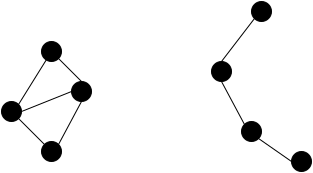
\includegraphics[width=4in]{twoSepNet.png}
	\caption{An example when two separate subnets formed}
	\label{fig:twoSepNet}
\end{figure}

As mentioned earlier, DFS algorithm need each \gn's neighbors list in order to properly perform. To obtain this information, after the random \gn placement, the program can access each node's coordinates. Assuming node 1 ($node_1$) has the coordinate of $(x_1, y_1)$ and node 2 ($node_2$) has the coordinate of $(x_2, y_2)$, the distance between $node_1$ and $node_2$ can be easily computed by the distance formula. Therefore, if we denote the distance between $node_1$ and $node_2$ is $d$, then $d = \sqrt{(x_1 - x_2)^2+(y_1 - y_2)^2}$. Now if we denote each \gn's WiFi range to be $R$, then $node_1$ and $node_2$ are neighbors when $d\leq R$. While $node_1$ and $node_2$ are not neighbors when $d > R$. We used this process to generate neighbors list for each \gn. In practice, the global access of each \gn's coordinate information is usually not easy to obtain. Thus, Hello packets are used to generate neighbors list for each \gn.

The work flow of our simulation control program is described below. 

\begin{itemize}
	\item Read in simulation environment parameters. 
	\item Create a source node and $n$ gossip nodes.
	\item The wireless ad-hoc network channel speed is set to be 1Mbps for all \gns.
	\item Create a special wireless ad-hoc network connection between a source node and a \gn and set its speed to be 11Mbps.
	\item Compute the side size of a square area for nodes placement.
	\item Randomly place all nodes in the square area
	\item Install basic energy source and \wf ~radio energy model on the \gns.
	\item Assign IP addresses to all nodes.
	\item Install adaptive fanout \gp and UDP client application ~on the \gns.
	\item Install gossip generator application and UDP server application on the \sn.
	\item Generate neighbors list for each \gn.
	\item Check topology connectivity using DFS algorithm.
	\item If the topology is disconnected somehow, terminate this simulation.
	\item If the topology is connected, start the simulation.
\end{itemize}

The link speed among \gns is set to be 1Mbps because it is sufficient to transmit a very small Data packet quickly. The link speed between the source node and one of the \gn ~is set to be 11Mbps because we want to make sure that source node does not become the bottleneck for the performance of our proposed \gp. Since all nodes including the source node are randomly placed in this area, we make sure that the \wf ~range of the \sn ~is large enough that it will always be able to reach any \gns. The \wf ~range of \gns ~is set to be 50m in order to control node's degree. 

As we stated earlier, the simulation will stop once any \gn's energy is depleted. From that point, the program will enter the data collection and process stage. At this stage, the program is trying to calculate the following data:

\begin{itemize}
	\item Message broadcast time (one output file per simulation)
	\item Average overhead per node per \msg ~(average within each simulation)
	\item Average energy consumption per node per \msg ~(average within each simulation)
	\item Network lifetime
\end{itemize}

For the \msg ~broadcast time, the program will access the vector stored in the \sn ~that represent the time stamps for each generated new broadcast \msg. Similarly, it will also access $n$ vectors from $n$ \gns. These vectors stored the received broadcast \msg ~time stamps of each \gn. Let's take a look at an example where we have one \sn ~and one \gn and the protocol successfully broadcast $m$ \msgs, if we denote the vector on the \sn ~side to be $T_s=<t_{s1}, t_{s2}, \ldots, t_{sm}>$ and the vector on the \gn ~side to be $T_g=<t_{g1}, t_{g2}, \ldots, t_{gm}>$, then the delay for these \msgs ~are $T_{delay}= T_g - T_s = <t_{g1}-t_{s1}, t_{g2}-t_{s2}, \ldots, t_{gm}-t_{sm}>$. For the scenario where $n$ \gns participated in the broadcasting process, because we are interested in \msg ~broadcast time, the program will first calculate the $T_{delay}$ for each \gn ($T_{delay_1},T_{delay_2},\ldots,T_{delay_n} $). Then it will loop through the first element in those vectors and store the maximum delay because by our definition for one broadcast \msg ~the time difference between the last \gn received the \msg ~and the time the \sn ~generate that \msg is the broadcast time for that \msg. And then the program will repeat that process until it reaches the $m_{th}$ broadcast \msg. However, we would like to point out that this process is only applied on a per simulation basis. To obtain the data that later our performance metrics need, further process need to be done.

For the overhead, we defined it as the total number of packets this protocol sent during the simulation. This includes Ack packet, Request packet, and Data packet. Our simulation control program first will access the \emph{packetSent} counter on each \gn. Then it will average over total number of broadcast \msgs ($m$ \msgs). Finally, it will take that number and average over number of \gns ~($n$ gossip nodes). Again, this process is done in a per simulation basis. Further data process is needed to yield our desired performance metrics data.

Similar to the process of calculating average overhead per node per \msg, in order to compute average energy consumption per node per \msg, the program would first collect consumed energy from the \gns, and then average over number of \gns ~($n$). And finally it will take that number and average over total number of broadcast \msgs ~($m$). 

The network lifetime is defined as the time duration which all \gns ~have energy to receive and transmit packets. Therefore, the program simply output the simulation stop time to a file.

\chapter{Performance Evaluation}
\label{Chapter5}
%\lhead{Chapter 5. \emph{Performance Evaluation}} % Write in your own chapter title to set the page header

In this chapter, we first will introduce our designed performance metrics in order to properly evaluate our proposed adaptive fanout \pp ~\gp. Then we will explain our simulation environment settings. Finally, we will analyze the simulation results.

\section{Performance Metrics} \label{pm}
As we stated in Section \ref{basic gossip}, the objective of our proposed approach is to achieve the balance between fast broadcasting time and long network lifetime. So obviously, the first two performance metrics that we proposed are \emph{Average \nl} and \emph{Average Message Broadcast Time}. Other performance metrics are \emph{Average Overhead Per Node Per Message}, \emph{Average Consumed Energy Per Node Per Message}, and \emph{Average Number of Success Broadcast Messages}.

\subsection{Average Network Lifetime}
%\textbf{Average Network Lifetime}

Before we define \emph{Average Network Lifetime}, we need to define \emph{Network Lifetime} first. 

\textbf{Network Lifetime}: The time duration which a wireless ad-hoc network can physically broadcast \msgs ~successfully.

When a \gn's energy is depleted, this \gn ~will no longer be able to transmit or receive new broadcast \msgs. Thus, this network is considered to be physically unable to broadcast \msgs ~successfully. Now the definition of \emph{Average Network Lifetime} is simply just an average over all \emph{Network Lifetime} under $n$ \gns ~case. For example, if we ran $s$ simulations under $n=10$ setting, and we denote \emph{Average Network Lifetime} for $10$ \gns ~as $L_{avg\_10}$, then the following equation can be used to calculate the \emph{Average Network Lifetime}.

\[ L_{avg\_10} =\frac{L_1 + L_2 + \ldots + L_{s}}{s} \]

This performance metric measures how long a wireless ad-hoc network with $n$ \gns ~can stay connected when running our proposed adaptive fanout \gp.

\subsection{Average Message Broadcast Time}
%\textbf{Average Message Broadcast Time}

Before we jump into the definition of \emph{Average Message Broadcast Time}, we first need to clearly define \emph{Message Broadcast Time}.

\textbf{Message Broadcast Time}: The maximum delay among \gns ~for each broadcast \msg.

Because here we are trying to measure the broadcast time of a certain \msg, it only makes sense when we sample the maximum delay among all \gns ~because the \msg ~received time of the last \gn ~determined our message broadcast time for a particular \msg. Now the \emph{Average Message Broadcast Time} is just an average over all \msg ~broadcast time under $n$ \gn ~case. Now because the randomness of our proposed \gp, each simulation under $n$ \gn ~case can result in different number of success broadcast \msgs. Therefore, for $n$ \gn ~case simulations, we first calculate the \emph{Average message broadcast time} for each simulation. And then we perform the average among those number to obtain this performance metrics data.

For example, let's denote the \emph{Average Message Broadcast Time} for $i$th simulation as $T_i$ and the \emph{Average Message Broadcast Time} for $n$ nodes as $T_{avg\_n}$. If we performed $s$ simulations, then the following equation can be used to calculate this metric:

\[ T_{avg\_n} = \frac{T_1 + T_2 + \ldots + T_s}{s} \]

This metric indicates the time needed for a broadcast \msg ~to reach every \gn ~in the network.

\subsection{Average Overhead Per Node Per Message}

The \emph{overhead} here is defined as the total number of packets sent by a \gn. These packets includes Ack packet, Request packet, and Data packet. For every simulation, in order to accurately measure the overhead for each \gn ~and for each broadcast \msg, we simply performed an average over $n$. And then take that number and further average over number of broadcast \msgs being sent. So for $k$th simulation, if we denote the overhead of node $i$ for \msg ~$j$ as $O_{ij}$, the number of \gns ~are $n$, and the system broadcast $m$ \msgs. Then for this simulation, the \emph{Average Overhead Per Node Per Message} can be computed using the following equation:

\[ O_{k} = \frac{(O_{11} + O_{21} + \ldots + O_{n1})  + \ldots + (O_{1m} + O_{2m} + \ldots + O_{nm})}{n\times m} \]

If we performed $s$ simulations under $n$ \gns ~setting, then the \emph{Average Overhead Per Node Per Message} among these simulations is:

\[ O_{avg\_n} = \frac{O_1 + O_2 + \ldots + O_s}{s} \]

%+ (O_{12} + O_{22} + \ldots + O_{n2})
%\mbox{Average Overhead Per Node Per Message}

This performance metric indicates how many packets are sent out for a \gn ~to facilitate broadcasting one \msg. 

\subsection{Average Energy Consumption Per Node Per Message}

This performance metric is quite self-explanatory. We measure the amount of energy consumed by each \gn ~during the simulation. Then we take that number and average among $m$ \msgs. $E_k$ is the \emph{Average Energy Consumption Per Node Per Message} for the $k$th simulation under $n$ \gns.

\[ E_k = \frac{E_{node\_1} + E_{node\_2} + \ldots + E_{node\_n}}{n\times m} \]

Now if we ran $s$ simulations, then \emph{Average Energy Consumption Per Node Per Message} under $n$ \gns ~can be calculated using the following equation:

\[ E_{avg\_n} = \frac{E_1 + E_2 + \ldots + E_s}{s} \]

This metric measures the amount of energy needed for a \gn ~to facilitate broadcasting one \msg. 

\subsection{Average Number of Broadcast Messages}

This metric measures how many \msgs ~can be successfully broadcast with limited energy sources. If we ran $s$ simulations under $n$ \gns ~setting, this metric can be computed using the following equation:

\[ N_{avg\_n} = \frac{N_1 + N_2 + \dots + N_s}{s} \]

\section{Simulation Environment Settings}

In order to properly evaluate our proposed \pp ~\gp, we need to compare it to the same basic \pp ~\gp ~but with constant \emph{Fanout} settings. Here we picked three typical \emph{Fanout} values. They are $f=1, 5, 10$. By obtaining performance metrics data from these three constant fanout settings, we can study how different \emph{Fanout} affect protocol performance. 

The simulation environment setting is summarized below.

\begin{itemize}
	\item Fanout: 1, 5, 10, or adaptive
	\item Number of nodes: 10, 50, 90, 130, 170
	\item \wf ~speed among \gns: 1Mbps
	\item \wf ~speed between the \sn ~and a \gn: 11Mbps
	\item MAC: IEEE 802.11 for \gns ~and \sn
	\item RTS/CTS: On
	\item Gossip node maximum \wf ~range: 50m
	\item Source node maximum \wf ~range: 500m
	\item Simulation stop time: 100000.0s
	\item Initial battery energy: 108.0J  (3V)
	\item Gossip interval: 1.0s
	\item Request interval 5.0s
	\item \wf ~radio idle current: 0.0A
	\item \wf ~radio sleep current: 0.0A
	\item \wf ~radio transmit current: 0.38A
	\item \wf ~radio receive current: 0.313A
	\item Gossip nodes IP address: 10.1.1.0/24
	\item Source node and a \gn's IP address: 10.1.2.0/24	
\end{itemize}

As we stated earlier, the simulation stop time is set to be large enough so that the energy sources on \gns ~will be depleted first. Thus, it will trigger the termination of our simulations. 

\section{Result Analysis}

In order to obtain simulation data for these settings, we ran 2000 simulations. Because of the random placement of \gns ~can potentially generate a disconnected topology, some of the simulations will be terminated in the beginning. Table \ref{table:sim} shows the number of successful simulations under each number of \gns ~setting. It is worth noting that this table holds true for all four \emph{Fanout} settings.

\begin{table}[h]
	\centering
	\caption{Number of Simulations Run}
	\label{table:sim}
	\begin{tabular}{|c|c|c|}
		\hline 
		Number of gossip nodes & Total number of simulations & Number of success simulations \\ 
		\hline 
		10 & 100 & 85 \\ 
		\hline 
		50 & 100 & 52 \\ 
		\hline 
		90 & 100 & 50 \\ 
		\hline 
		130 & 100 & 46 \\ 
		\hline 
		170 & 100 & 34 \\ 
		\hline 
	\end{tabular} 
\end{table}

By conducting statistical analysis based on the method in Section \ref{pm}, we were able to extract the data of each performance metrics. 

Figure \ref{fig:brTime} depicts the \emph{Average Message Broadcast Time} over number of \gns. As we would expect, under any \emph{Fanout} setting, the \emph{\ambt} will increase as the number of \gns ~increase. It is especially obvious for $f=1$ setting. For other \emph{Fanout} settings, their \emph{\ambt} are much shorter than $f=1$ setting across different number of \gns ~settings. We can see a huge performance improvement when \emph{Fanout} is switched from 1 to 5. That is because a \gn ~can forward the broadcast \msg ~to more neighbors comparing to $f=1$ setting. However, the performance improvement from $f=5$ to $f=10$ is marginal. We believe that it is related to the average node's degree since a \emph{Fanout} setting that exceeds the number of neighbors a \gn ~has will bring no additional performance boost. Our adaptive fanout approach performed as good as $f=5$ setting even though its \emph{Fanout} is ranging from 1 to 5 during a simulation. 

\begin{figure} 
	\centering
	\includegraphics[width=5.5in]{brTime.png}
	\caption{Average message broadcast time vs. number of nodes}
	\label{fig:brTime}
\end{figure}

Figure \ref{fig:life} presents the \emph{Average Network Lifetime} over different number of \gns. For three constant \emph{Fanout} settings, the \emph{\anl} decreases as \emph{Fanout} increases. This is within our expectation because for every gossip round, a \gn ~with a higher \emph{Fanout} setting will have to contact more neighbors thus consume more energy. $f=1$ setting has the best \emph{\anl} but as we see in Figure \ref{fig:brTime}, it has the worst \emph{\ambt}. Under $f=5$ setting, the \emph{\anl} is reasonably good while the \emph{\ambt} is shorter. However, our proposed adaptive fanout setting can achieve even better \emph{\anl} comparing to $f=5,10$ settings while still perform as good as the other two in terms of \emph{\ambt}. 

\begin{figure} 
	\centering
	\includegraphics[width=5.5in]{life.png}
	\caption{Average network lifetime vs. number of nodes}
	\label{fig:life}
\end{figure}

From Figure \ref{fig:energy}, we can see that as number of \gns ~increases, the \emph{Average Energy Consumption Per Node Per Message} increases as expected. For the ease of discussion, in the following chapter we will call it \emph{Average Energy Consumption}. The interesting part here we would like to point out is that $f=1$ setting actually has the highest energy consumption. The reason is that even though it has the longest \emph{\anl}, it also has the worst \emph{\ambt}. So given these two constrains, the number of \msgs it can broadcast is less than other \emph{Fanout} settings. Since we computed this metric on a per \msg ~basis, it would result in a higher \emph{\aec}. Under $f=5$ and adaptive fanout setting, their \emph{\aec} plots are almost overlapping each other. The reason is the trade off between \emph{\ambt} and \emph{\anl}. $f=10$ setting has the lowest \emph{\aec} except for 170 \gns ~setting, but as shown in Figure \ref{fig:life}, it has the worst \emph{\anl}. 

\begin{figure} 
	\centering
	\includegraphics[width=5.5in]{energy.png}
	\caption{Average consumed energy per node per message vs. number of nodes}
	\label{fig:energy}
\end{figure}

Figure \ref{fig:overhead} shows the results of \emph{Average Overhead Per Node Per Message} over various number of \gns. For the ease of discussion, from now on we will call it \emph{\ao}. Comparing Figure \ref{fig:overhead} to Figure \ref{fig:energy}, we can see that the shape of each plot is almost identical even though the unit on the y-axis is different. That is because energy consumption is closely related to overhead since overhead is defined as the number of packets sent by each \gn. Therefore, the same analysis on Figure \ref{fig:energy} can be applied here as well.

\begin{figure} 
	\centering
	\includegraphics[width=5.5in]{overhead.png}
	\caption{Average overhead per node per message vs. number of nodes}
	\label{fig:overhead}
\end{figure}

Lastly, Figure \ref{fig:brNum} presents the number of \msgs broadcast over different number of \gns. $f=1$ setting can deliver the least amount of \msgs comparing to other \emph{Fanout} settings. In general, higher \emph{Fanout} setting will increase the number of \msgs the protocol can deliver. However, as we see in Figure \ref{fig:brTime}, switching \emph{Fanout} from 5 to 10 would result in a very limited performance boost. Our proposed adaptive fanout approach performed as good as $f=5,10$ setting while as shown in Figure \ref{fig:life} it has longer \emph{\anl}.

\begin{figure} 
	\centering
	\includegraphics[width=5.5in]{brNum.png}
	\caption{Average number of broadcast messages vs. number of nodes}
	\label{fig:brNum}
\end{figure}

\chapter{Conclusions and Future Work}
\label{Chapter6}
%\lhead{Chapter 6. \emph{Conclusions and Future Work}} % Write in your own chapter title to set the page header

In this thesis, we introduced research progress in gossip techniques for wireless broadcasting in recently years. We pointed out that despite all these efforts dedicated into reduing gossip broadcasting protocol overhead, very little research has focused on energy efficiency and network lifetime. Those aspect used to be not very important when designing new broadcasting protocols because nodes usually have stable power. However, with the emergence of Internet of Things (IoT) devices, broadcasting protocols that take energy consumption  into account and optimizing it will be favored over those that do not. Based on our observation of the tradeoff between battery life and broadcasting time regarding \emph{Fanout} parameter, we proposed a new energy-aware gossip broadcasting protocol that could balance between network lifetime and broadcasting time. In order to evaluate the performance of our proposed approach, we designed several metrics and we developed the protocol in open-source software ns-3. Simulation results showed that comparing to constant $f=5$ setting, our adaptive approach significantly extended network lifetime while only performed slightly slower in term of message broadcasting time. We suspect the casue for marginal performance improvements for $f=10$ setting comparing to $f=5$ setting is the average node's degree. In other words, very little performance boost can be observed when \emph{Fanout} is set beyond average node's degree since a node simply cannot reach out to 10 neighbors when it only has 5 neighbors. As we discussed earlier, $f=1$ setting has the worst message broadcasting time. But on the flip side, it would result in a longest network lifetime which could be desirable for some applications. 

In conclusion, our proposed energy-aware adaptive gossip broadcasting protocol can leverage the advantages of low \emph{Fanout} setting and high \emph{Fanout} setting. Thus, we can extend network lifetime while still perform as good as high \emph{Fanout} setting in term of broadcasting time. Constant $f=1$ setting is recommended for networks that consists of nodes with strict energy constrain. 

For future work, we would like to use multicast instead of multiple unicast for each node to send the new message. The reason is that if we assume $X J$ is the amount of energy used to transmit a packet for a sender, and $f=5$, one multicast will only consum $X J$ while five unicast will consum $5X J$. Another interesting scenerio would be to set very different initial energy but same battery capacity for each node. Thus each node would be operating at different \emph{Fanout} setting from the begining due to different remaining energy fraction. We believe this would better capture the advantage of our proposed appraoch over constant \emph{Fanout} setting.


%\chapter{Introduction}
%I have done some excellent research.
%\section{Introduction to the Introduction}
%\begin{figure}[!ht]
%\centering
%\fbox{\huge Box}
%\caption{Go figure.}
%\end{figure}

%\chapter{The Body}
%This is the meat.
%\section{Meat}
%We're born meat and we die meat. Meanwhile, we learn (see Algorithm \ref{alg:learning}).
%
%\begin{algorithm}[h]
%\caption{\textsc{Learning}}
%\label{alg:learning}
%\begin{algorithmic}[1]
%\ENSURE{Optimal policy $\mathcal{C}$}
%	\STATE $\mathcal{C} \gets 42$
%	\RETURN $\mathcal{C}$
%\end{algorithmic}
%\end{algorithm}
%
%\chapter{Conclusion}
%Wow, that really was excellent.
%\section{Fin}
%This is the end, my only friend, the end.


\bibliographystyle{plain}
\bibliography{thesis}

%\appendix
%\chapter{Redundancy}
%This appendix is inoperable.

\end{document}
